%!TeX root=../tese.tex
%("dica" para o editor de texto: este arquivo é parte de um documento maior)
% para saber mais: https://tex.stackexchange.com/q/78101/183146

%% ------------------------------------------------------------------------- %%
\chapter{Delimitações inferiores de Wilber}
\label{cap:wilber}

\definecolor{vibrantRed}{HTML}{FF4136}
\definecolor{electricBlue}{HTML}{0074D9}
\definecolor{limeGreen}{HTML}{2ECC40}
\definecolor{brightOrange}{HTML}{FF851B}

Aqui irei deixar algumas imagens das delimitações de wilber utilizadas no pôster que serão utilizadas na minha tese do TCC em breve! :)

oioi 

O primeiro grande avanço na área de delimitar custo 


oio

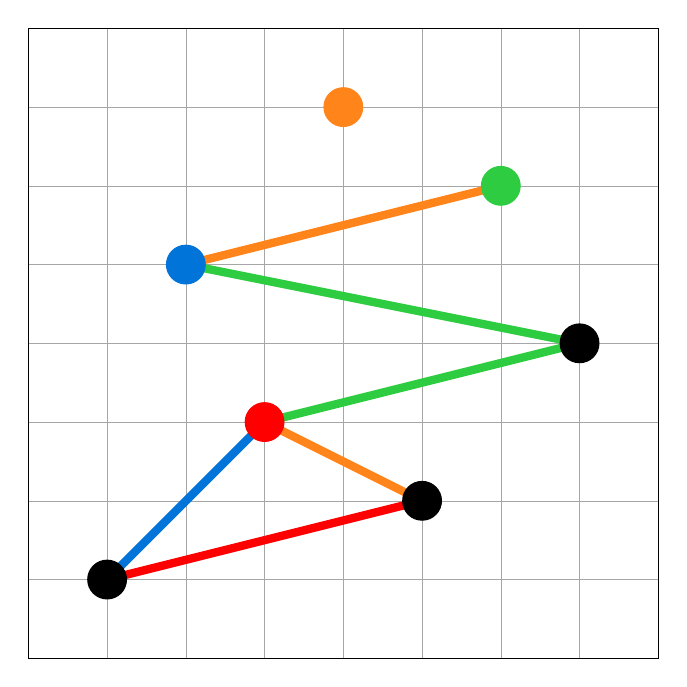
\begin{tikzpicture}[scale=1]
    \draw[very thin, gray!70] (0,0) grid (8,8);
    
    %\draw[black, line width=1pt] (3,1) -- (8,2) -- (10,3) -- (9,8);
    %\draw[black, line width=1pt] (3,1) -- (2,6) -- (1,9);
    %\draw[black, line width=1pt] (8,2) -- (4,4) -- (5,5) -- (6,7) -- (7,10);
    
    %\draw[red, line width=3pt] (3,3) -- (3,0);
    \draw[red, line width=3pt] (1,1) -- (5,2);
    
    
    %\draw[electricBlue, line width=3pt] (2,5) -- (2,0);
    \draw[electricBlue, line width=3pt] (1,1) -- (3,3);
    
    
    %\draw[limeGreen, line width=3pt] (6,6) -- (6,0);
    \draw[limeGreen, line width=3pt] (2,5) -- (7,4) -- (3,3);

    %\draw[brightOrange, line width=3pt] (4,7) -- (4,0);
    \draw[brightOrange, line width=3pt] (2,5) -- (6,6);
    \draw[brightOrange, line width=3pt] (3,3) -- (5,2);

    \filldraw[black] (1,1) circle (7pt);
    \filldraw[black] (5,2) circle (7pt);
    \filldraw[red] (3,3) circle (7pt);
    \filldraw[black] (7,4) circle (7pt);
    \filldraw[electricBlue] (2,5) circle (7pt);
    \filldraw[limeGreen] (6,6) circle (7pt);
    \filldraw[brightOrange] (4,7) circle (7pt);
    \draw[black, line width=0.5pt] (0,0) rectangle (8,8);
\end{tikzpicture}

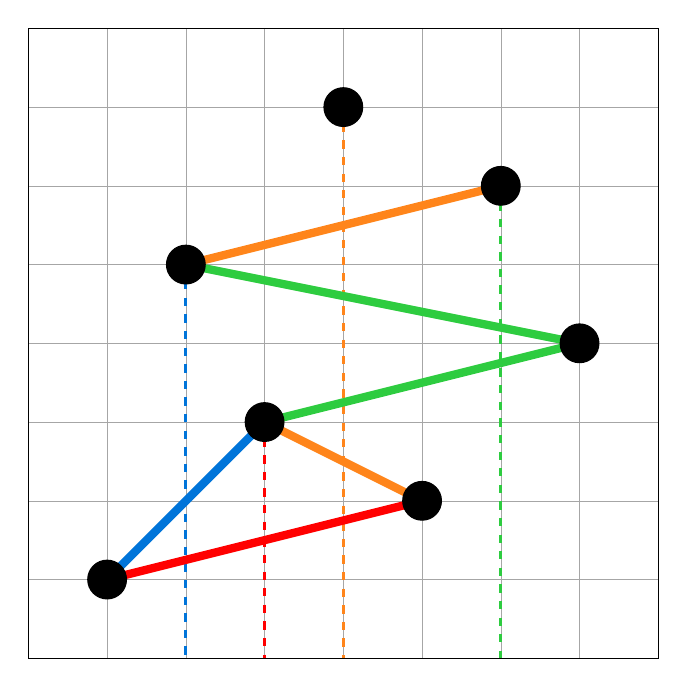
\begin{tikzpicture}[scale=1]
    \draw[very thin, gray!70] (0,0) grid (8,8);
    
    \draw[dashed, brightOrange, line width=1pt] (4,7) -- (4,0);
    \draw[dashed, red, line width=1pt] (3,3) -- (3,0);
    \draw[dashed, limeGreen, line width=1pt] (6,6) -- (6,0);
    \draw[dashed, electricBlue, line width=1pt] (2,5) -- (2,0);

    \draw[red, line width=3pt] (1,1) -- (5,2);
    
    \draw[electricBlue, line width=3pt] (1,1) -- (3,3);
    
    \draw[limeGreen, line width=3pt] (2,5) -- (7,4) -- (3,3);

    \draw[brightOrange, line width=3pt] (2,5) -- (6,6);
    \draw[brightOrange, line width=3pt] (3,3) -- (5,2);

    \filldraw[black] (1,1) circle (7pt);
    \filldraw[black] (5,2) circle (7pt);
    \filldraw[black] (3,3) circle (7pt);
    \filldraw[black] (7,4) circle (7pt);
    \filldraw[black] (2,5) circle (7pt);
    \filldraw[black] (6,6) circle (7pt);
    \filldraw[black] (4,7) circle (7pt);
    \draw[black, line width=0.5pt] (0,0) rectangle (8,8);
\end{tikzpicture}


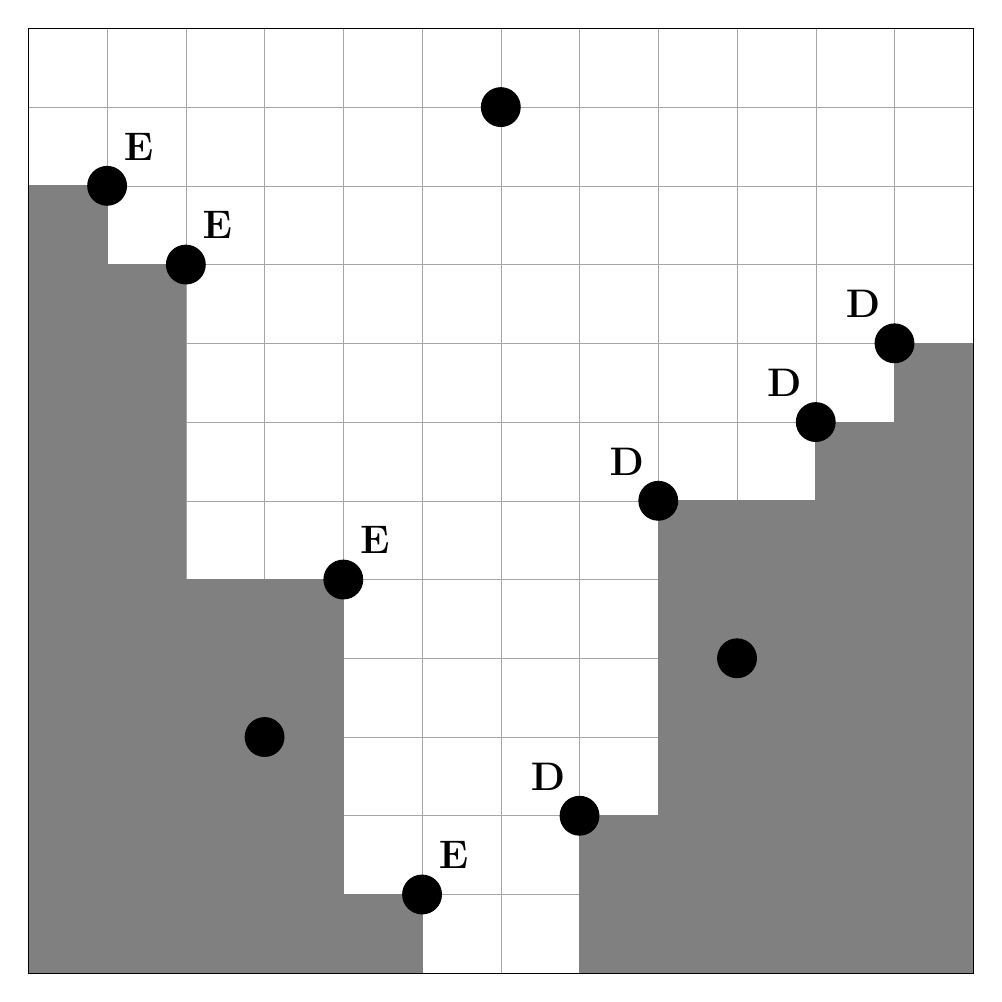
\begin{tikzpicture}[scale=1]
    \draw[very thin, gray!70] (0,0) grid (12,12);
    
    \draw[fill=gray, gray] (0,0) rectangle (1,10);
    \draw[fill=gray, gray] (1,0) rectangle (2,9);
    \draw[fill=gray, gray] (2,0) rectangle (4,5);
    \draw[fill=gray, gray] (4,0) rectangle (5,1);


    \draw[fill=gray, gray] (11,8) rectangle (12,0);
    \draw[fill=gray, gray] (10,7) rectangle (11,0);
    \draw[fill=gray, gray] (8,6) rectangle (10,0);
    \draw[fill=gray, gray] (7,2) rectangle (8,0);


    %\draw[red, line width=2pt] (6,11) -- (6,0);
    

    \filldraw[black] (5,1) circle (7pt);
    \filldraw[black] (7,2) circle (7pt);
    \filldraw[black] (3,3) circle (7pt);
    \filldraw[black] (9,4) circle (7pt);
    \filldraw[black] (4,5) circle (7pt);
    \filldraw[black] (8,6) circle (7pt);
    \filldraw[black] (10,7) circle (7pt);
    \filldraw[black] (11,8) circle (7pt);
    \filldraw[black] (2,9) circle (7pt);
    \filldraw[black] (1,10) circle (7pt);
    \filldraw[black] (6,11) circle (7pt);

    \node at (1.4,10.5) {\textbf{\Large E}};
    \node at (2.4,9.5) {\textbf{\Large E}};
    \node at (4.4,5.5) {\textbf{\Large E}};
    \node at (5.4,1.5) {\textbf{\Large E}};

    \node at (10.6,8.5) {\textbf{\Large D}};
    \node at (9.6,7.5) {\textbf{\Large D}};
    \node at (7.6,6.5) {\textbf{\Large D}};
    \node at (6.6,2.5) {\textbf{\Large D}};


    \draw[black, line width=0.5pt] (0,0) rectangle (12,12);
\end{tikzpicture}

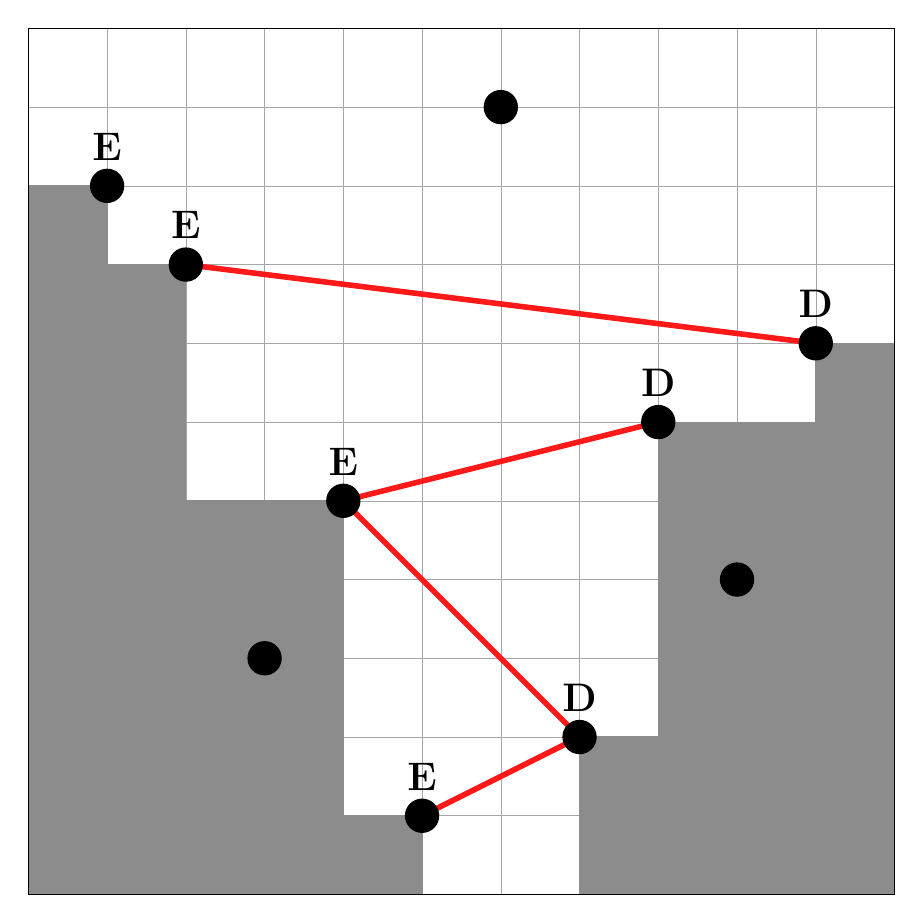
\begin{tikzpicture}[scale=1]
    \draw[very thin, gray!70] (0,0) grid (11,11);
    
    \draw[fill=gray!90, gray!90] (0,0) rectangle (1,9);
    \draw[fill=gray!90, gray!90] (1,0) rectangle (2,8);
    \draw[fill=gray!90, gray!90] (2,0) rectangle (4,5);
    \draw[fill=gray!90, gray!90] (4,0) rectangle (5,1);

    \draw[red!90, line width=2pt] (2,8) -- (10,7);
    \draw[red!90, line width=2pt] (8,6) -- (4,5) -- (7,2) -- (5,1);

    %\draw[fill=gray!90, gray!90] (11,8) rectangle (12,0);
    \draw[fill=gray!90, gray!90] (10,7) rectangle (11,0);
    \draw[fill=gray!90, gray!90] (8,6) rectangle (10,0);
    \draw[fill=gray!90, gray!90] (7,2) rectangle (8,0);    

    \filldraw[black] (5,1) circle (6pt);
    \filldraw[black] (7,2) circle (6pt);
    \filldraw[black] (3,3) circle (6pt);
    \filldraw[black] (9,4) circle (6pt);
    \filldraw[black] (4,5) circle (6pt);
    \filldraw[black] (8,6) circle (6pt);
    \filldraw[black] (10,7) circle (6pt);
    \filldraw[black] (2,8) circle (6pt);
    \filldraw[black] (1,9) circle (6pt);
    \filldraw[black] (6,10) circle (6pt);


    \node at (1,9.5) {\textbf{\Large E}};
    \node at (2,8.5) {\textbf{\Large E}};
    \node at (4,5.5) {\textbf{\Large E}};
    \node at (5,1.5) {\textbf{\Large E}};

    \node at (10,7.5) {\textbf{\Large D}};
    \node at (8,6.5) {\textbf{\Large D}};
    \node at (7,2.5) {\textbf{\Large D}};


    \draw[black, line width=0.5pt] (0,0) rectangle (11,11);
\end{tikzpicture}

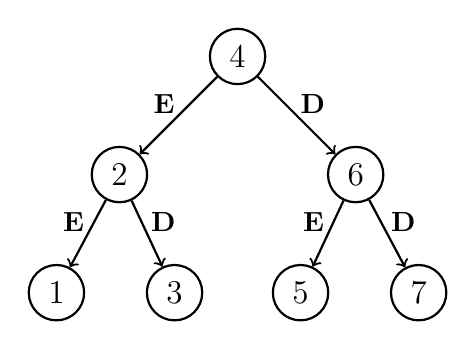
\begin{tikzpicture}
    [node/.style={circle,draw,minimum size=2em, thick, font=\large}]
    \node[node] (D) at (0,0) {$4$};
    \node[node] (B) at (-1.5,-1.5) {$2$};
    \node[node] (A) at (-2.3,-3) {$1$};
    \node[node] (C) at (-0.8,-3) {$3$};
    \node[node] (E) at (0.8,-3) {$5$};
    \node[node] (F) at (1.5,-1.5) {$6$};
    \node[node] (G) at (2.3,-3) {$7$};
    
    \draw[thick, ->] (D) -- (B) node[midway, left, yshift=0.15cm, xshift=0.08cm] {\textbf{E}};
    \draw[thick, ->] (B) -- (A) node[midway, left, yshift=0.15cm, xshift=0.08cm] {\textbf{E}};
    \draw[thick, ->] (B) -- (C) node[midway, right, yshift=0.15cm, xshift=-0.08cm] {\textbf{D}};
    
    \draw[thick, ->] (D) -- (F) node[midway, right, yshift=0.15cm, xshift=-0.08cm] {\textbf{D}};
    \draw[thick, ->] (F) -- (E) node[midway, left, yshift=0.15cm, xshift=0.08cm] {\textbf{E}};
    \draw[thick, ->] (F) -- (G) node[midway, right, yshift=0.15cm, xshift=-0.08cm] {\textbf{D}};

\end{tikzpicture}

\renewcommand{\arraystretch}{1.5}

\begin{tabular}{>{\centering\arraybackslash}p{0.7cm} >{\centering\arraybackslash}p{5cm} p{0.3cm}} % Define as larguras das colunas
    Nó & Alternância de filhos & \# \\
    \hline
    2 & E, D  & 1 \\
    4  & E, D, E, D, E, D  & 5  \\
    6  & E, D  & 1  \\
    \hline
    Total  &   & 7  \\
\end{tabular}

%\begin{tikzpicture}[
%    level distance=1.5cm,
%    level 1/.style={sibling distance=4cm},
%    level 2/.style={sibling distance=2cm},
%    every node/.style={circle, draw, minimum size=8mm, inner sep=0pt, font=\large},
%    edge from parent/.style={draw},
%    edge from parent path={(\tikzparentnode) -- (\tikzchildnode)},
%    triangle/.style={isosceles triangle, isosceles triangle apex angle=60, shape border rotate=90, draw, minimum height=10mm, minimum width=10mm}, % Orientando para cima
%    triangle text/.style={font=\large, text centered, anchor=center} % Centralizando o texto
%    ]
%    \node {8}
%      child {node {3}
%        child {node {1}}
%        child {node {6}
%          child {node {4}}
%          child {node {7}
%            child {node[triangle] {z}} % Adiciona o triângulo com o texto no meio
%            child {node[triangle] {z}}}}} % Adiciona o triângulo com o texto no meio
%      child {node {10}
%        child[missing] {}
%        child {node {14}
%          child {node {13}}
%          child[missing] {}}};
          
%\end{tikzpicture}

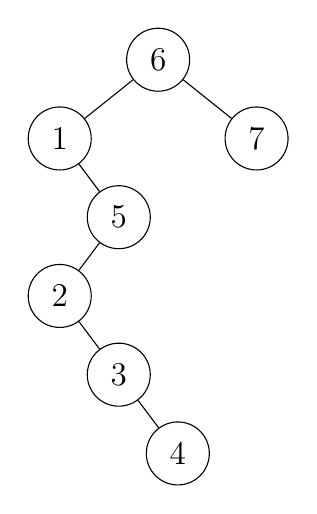
\begin{tikzpicture}[
    level distance=1cm,
    level 1/.style={sibling distance=2.5cm},
    level 2/.style={sibling distance=1.5cm},
    every node/.style={circle, draw, minimum size=8mm, inner sep=0pt, font=\large},
    edge from parent/.style={draw},
    edge from parent path={(\tikzparentnode) -- (\tikzchildnode)},
    triangle/.style={isosceles triangle, isosceles triangle apex angle=60, shape border rotate=90, draw, minimum height=10mm, minimum width=10mm}, % Orientando para cima
    triangle text/.style={font=\large, text centered, anchor=center} % Centralizando o texto
    ]
    \node {6}
      child {node {1}
        child[missing] {}
        child {node {5}
          child {node {2}{
            child[missing] {}
            child {node {3}{
                child[missing] {}
                child {node {4}{}
            }
            }}
          }}
          child[missing] {}}} % Adiciona o triângulo com o texto no meio
      child {node {7}};
\end{tikzpicture}

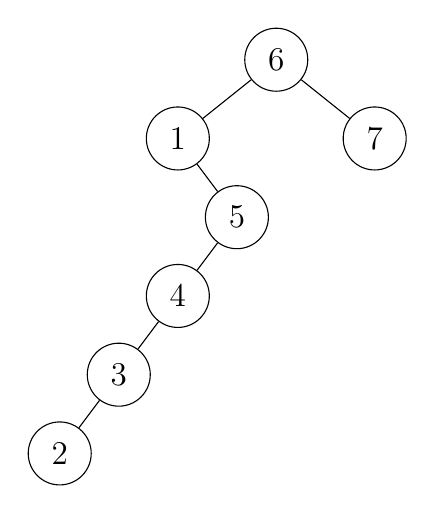
\begin{tikzpicture}[
    level distance=1cm,
    level 1/.style={sibling distance=2.5cm},
    level 2/.style={sibling distance=1.5cm},
    every node/.style={circle, draw, minimum size=8mm, inner sep=0pt, font=\large},
    edge from parent/.style={draw},
    edge from parent path={(\tikzparentnode) -- (\tikzchildnode)},
    triangle/.style={isosceles triangle, isosceles triangle apex angle=60, shape border rotate=90, draw, minimum height=10mm, minimum width=10mm}, % Orientando para cima
    triangle text/.style={font=\large, text centered, anchor=center} % Centralizando o texto
    ]
    \node {6}
      child {node {1}
        child[missing] {}
        child {node {5}
          child {node {4}{
            child {node {3}{
                child {node {2}{}}
                child[missing] {}
            }}
            child[missing] {}
          }}
          child[missing] {}}} 
      child {node {7}};
\end{tikzpicture}

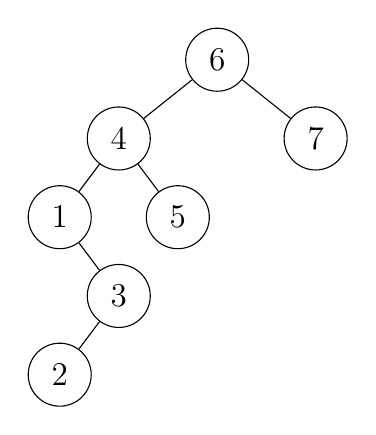
\begin{tikzpicture}[
    level distance=1cm,
    level 1/.style={sibling distance=2.5cm},
    level 2/.style={sibling distance=1.5cm},
    every node/.style={circle, draw, minimum size=8mm, inner sep=0pt, font=\large},
    edge from parent/.style={draw},
    edge from parent path={(\tikzparentnode) -- (\tikzchildnode)},
    triangle/.style={isosceles triangle, isosceles triangle apex angle=60, shape border rotate=90, draw, minimum height=10mm, minimum width=10mm}, % Orientando para cima
    triangle text/.style={font=\large, text centered, anchor=center} % Centralizando o texto
    ]
    \node {6}
      child {node {4}
        child {node {1}
          child[missing] {}
          child {node {3}
            child {node {2}}
            child[missing] {}}}
        child {node {5}}}
      child {node {7}};
\end{tikzpicture}

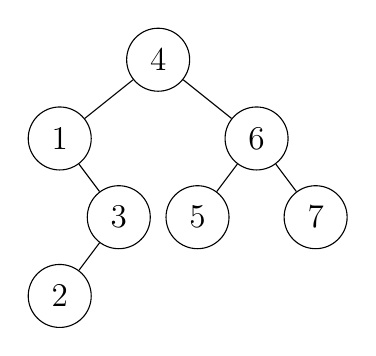
\begin{tikzpicture}[
    level distance=1cm,
    level 1/.style={sibling distance=2.5cm},
    level 2/.style={sibling distance=1.5cm},
    every node/.style={circle, draw, minimum size=8mm, inner sep=0pt, font=\large},
    edge from parent/.style={draw},
    edge from parent path={(\tikzparentnode) -- (\tikzchildnode)},
    triangle/.style={isosceles triangle, isosceles triangle apex angle=60, shape border rotate=90, draw, minimum height=10mm, minimum width=10mm}, % Orientando para cima
    triangle text/.style={font=\large, text centered, anchor=center} % Centralizando o texto
    ]
    \node {4}
      child {node {1}
        child[missing] {}
        child {node {3}
          child {node {2}}
          child[missing] {}}}
      child {node {6}
        child {node {5}}
        child {node {7}}};
\end{tikzpicture}


\begin{figure}[ht]
    \centering
    
    % Primeira linha de imagens
    \begin{minipage}{0.45\textwidth}
        \centering
        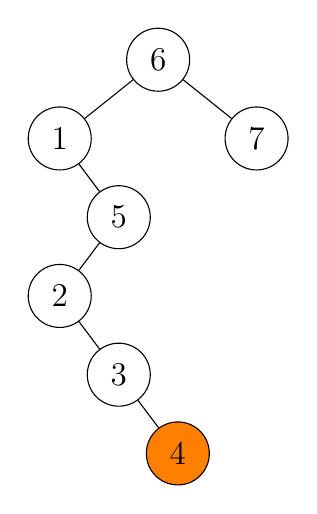
\begin{tikzpicture}[
            level distance=1cm,
            level 1/.style={sibling distance=2.5cm},
            level 2/.style={sibling distance=1.5cm},
            every node/.style={circle, draw, minimum size=8mm, inner sep=0pt, font=\large},
            edge from parent/.style={draw},
            edge from parent path={(\tikzparentnode) -- (\tikzchildnode)}
            ]
            \node {6}
              child {node {1}
                child[missing] {}
                child {node {5}
                  child {node {2}{
                    child[missing] {}
                    child {node {3}{
                        child[missing] {}
                        child {node[fill=orange] {4}{}
                    }
                    }}
                  }}
                  child[missing] {}}} 
              child {node {7}};
        \end{tikzpicture}
    \end{minipage}
    \hspace{1cm} % Espaço entre as imagens
    \begin{minipage}{0.45\textwidth}
        \centering
        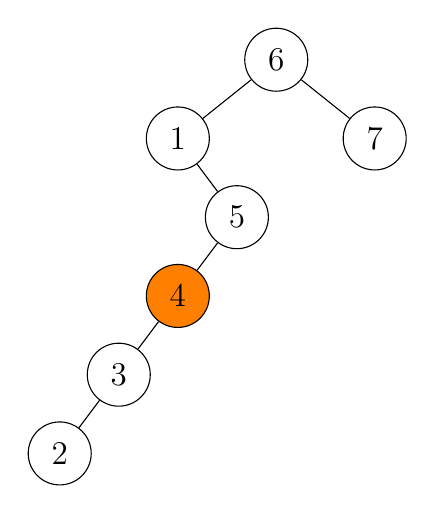
\begin{tikzpicture}[
            level distance=1cm,
            level 1/.style={sibling distance=2.5cm},
            level 2/.style={sibling distance=1.5cm},
            every node/.style={circle, draw, minimum size=8mm, inner sep=0pt, font=\large},
            edge from parent/.style={draw},
            edge from parent path={(\tikzparentnode) -- (\tikzchildnode)}
            ]
            \node {6}
              child {node {1}
                child[missing] {}
                child {node {5}
                  child {node[fill=orange] {4}{
                    child {node {3}{
                        child {node {2}{}}
                        child[missing] {}
                    }}
                    child[missing] {}
                  }}
                  child[missing] {}}} 
              child {node {7}};
        \end{tikzpicture}
    \end{minipage}
    
    \vspace{1cm} % Espaço entre as linhas
    
    % Segunda linha de imagens
    \begin{minipage}{0.45\textwidth}
        \centering
        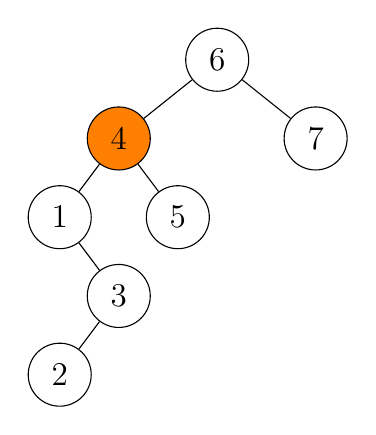
\begin{tikzpicture}[
            level distance=1cm,
            level 1/.style={sibling distance=2.5cm},
            level 2/.style={sibling distance=1.5cm},
            every node/.style={circle, draw, minimum size=8mm, inner sep=0pt, font=\large},
            edge from parent/.style={draw},
            edge from parent path={(\tikzparentnode) -- (\tikzchildnode)}
            ]
            \node {6}
              child {node[fill=orange] {4}
                child {node {1}
                  child[missing] {}
                  child {node {3}
                    child {node {2}}
                    child[missing] {}}}
                child {node {5}}}
              child {node {7}};
        \end{tikzpicture}
    \end{minipage}
    \hspace{1cm} % Espaço entre as imagens
    \begin{minipage}{0.45\textwidth}
        \centering
        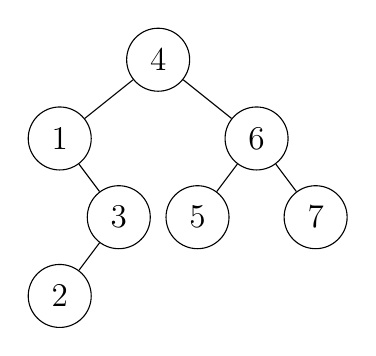
\begin{tikzpicture}[
            level distance=1cm,
            level 1/.style={sibling distance=2.5cm},
            level 2/.style={sibling distance=1.5cm},
            every node/.style={circle, draw, minimum size=8mm, inner sep=0pt, font=\large},
            edge from parent/.style={draw},
            edge from parent path={(\tikzparentnode) -- (\tikzchildnode)}
            ]
            \node {4}[fill=orange]
              child {node {1}
                child[missing] {}
                child {node {3}
                  child {node {2}}
                  child[missing] {}}}
              child {node {6}
                child {node {5}}
                child {node {7}}};
        \end{tikzpicture}
    \end{minipage}
    
    \vspace{1cm} % Espaço entre as linhas

    % Setas entre as imagens
    %\begin{tikzpicture}[overlay, remember picture]
        %\draw[->] (0,0) -- (3,0) node[midway, above] {};
        %\draw[->] (0,-4) -- (3,-4) node[midway, above] {};
        %\draw[->] (-3,-3) -- (-5.5,-5.5) node[midway, above] {};
    %\end{tikzpicture}

\end{figure}



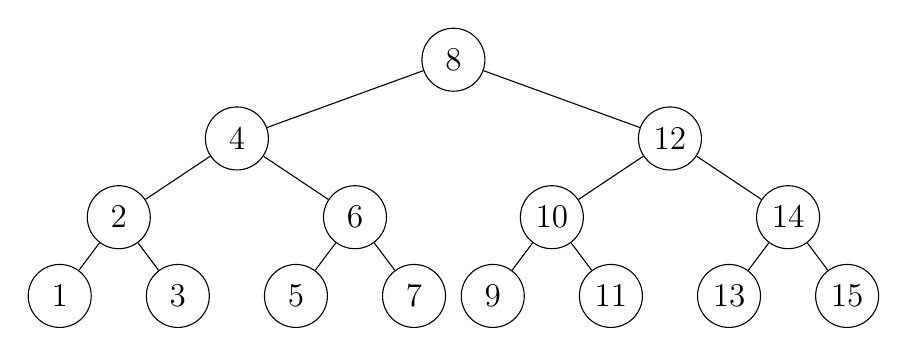
\begin{tikzpicture}[
  level distance=1cm,
  level 1/.style={sibling distance=5.5cm},
  level 2/.style={sibling distance=3cm},
  level 3/.style={sibling distance=1.5cm},
  every node/.style={circle, draw, minimum size=8mm, inner sep=0pt, font=\large},
  edge from parent/.style={draw},
  edge from parent path={(\tikzparentnode) -- (\tikzchildnode)}
  ]
  \node {8}
    child {node {4}
      child {node {2}
        child {node {1}}
        child {node {3}}}
      child {node {6}
        child {node {5}}
        child {node {7}}}}
    child {node {12}
      child {node {10}
        child {node {9}}
        child {node {11}}}
      child {node {14}
        child {node {13}}
        child {node {15}}}};
\end{tikzpicture}

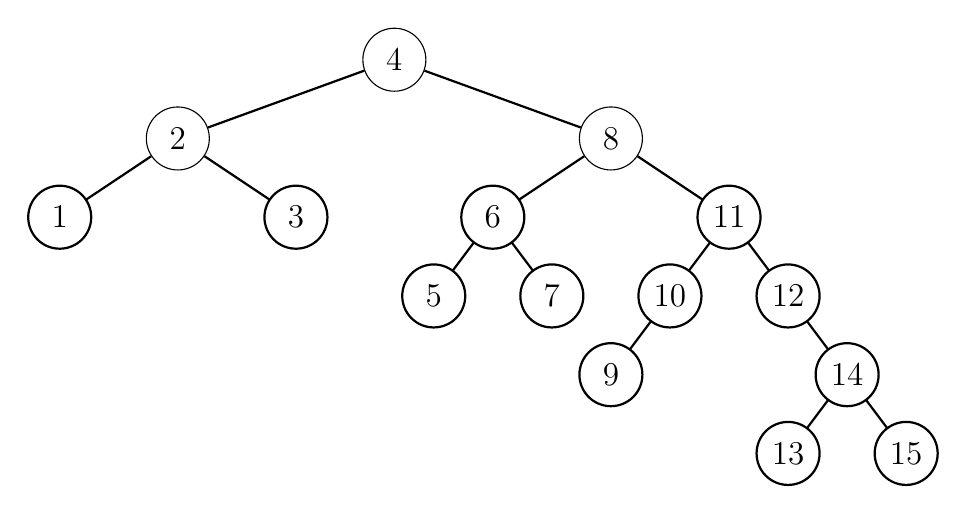
\begin{tikzpicture}[
  level distance=1cm,
  level 1/.style={sibling distance=5.5cm},
  level 2/.style={sibling distance=3cm},
  level 3/.style={sibling distance=1.5cm},
  every node/.style={circle, draw, minimum size=8mm, inner sep=0pt, font=\large},
  edge from parent/.style={draw, thick}, % Estilo padrão para arestas
  nodeRed/.style={circle, draw, minimum size=8mm, inner sep=0pt, font=\large, fill=red!20},
  nodeBlue/.style={circle, draw, minimum size=8mm, inner sep=0pt, font=\large, fill=blue!20}
  edge from parent/.style={draw},
  edge from parent path={(\tikzparentnode) -- (\tikzchildnode)}
  ]
  \node {4}
    child {node {2}
      child {node {1}}
      child {node {3}}}
    child {node {8}
      child {node {6}
        child {node {5}}
        child {node {7}}}
      child {node {11}
        child {node {10}
          child {node{9}}
          child[missing] {}}
        child {node {12}
          child[missing] {}
          child {node {14}
            child {node{13}}
            child {node {15}}}}}};
          %child {node {15}}}}};
\end{tikzpicture}

